%\chapter{Introduction}
\label{chap:intro}
\section{Motivation}

Significant advancements in micro- and nanotechnologies have enabled controlling heat flow in microscopic and even atomistic scale \cite{cahill03,cahill14}. Such thermal engineering has allowed, e.g. increasing the efficiency of thermoelectric heat-to-electricity converters \cite{snyder08,vineis10,shakouri11}, designing nanoporous aerogels for thermal insulation in buildings \cite{baetens11} and spacecraft \cite{jones06}, and mitigating the problem of overheating in microprocessors \cite{pop10}. Accurate temperature control is expected to generate also completely new technologies such as phase-change memory \cite{lankhorst05}, heat-assisted magnetic recording \cite{challener09}, tumor therapy based on nanoparticle heating \cite{avedisian09}, and information processing using thermal energy \cite{li12_rmp}. % For all such applications, a solid understanding of energy transfer processes in nanoscale is necessary. 

Microscopically, energy is transferred in solid-state systems by lattice vibrations, electromagnetic fields, and electrons \cite{chen}. Compared to macroscale, where energy transfer is characterized by constitutive material parameters such as thermal conductivity, energy transfer in nanoscale is enriched by the presence of intrinsic length scales competing with the system size \cite{chen}. For example, when the the scattering length or the wavelength of heat carriers is of the same order as the system size, classical laws such as Fourier's law of thermal conduction \cite{fourier} and Planck's law of thermal radiation \cite{planck00a} break down, giving rise to novel phenomena such as thermal conductance quantization \cite{rego98,angelescu98,schwab00} and near-field enhancement of thermal radiation \cite{volokitin07}. The technological prospects of nanostructures arise from the possibility to utilize such phenomena to design materials and devices with tailored properties. 

Due to the complexity of microscopic mathematical theory and the rich variety of phenomena present in nanoscale energy transfer, numerical simulations are invaluable tools in understanding and designing experimental measurements and guiding the design of more efficient materials and devices. Therefore, there is a growing need for powerful computational models delivering qualitative as well as quantitative insight into nanoscale energy transfer in different systems and conditions. 

\section{Scope and objectives}

This doctoral thesis aims at developing the physical insight needed to describe the microscopic aspects of energy transfer in nanoscale systems. To this end, we develop new computational tools and methods for atomic scale energy transfer simulations. The main focus areas of the thesis are modeling heat transfer by lattice waves (phonons\footnote{Throughout the thesis, we refer to lattice vibrations loosely as phonons, which are the quanta of vibrational eigenmode oscillations \cite{ziman}.}) in various geometries and developing quantum-mechanical computational methods for describing vibrational, electromagnetic as well as electronic energy transfer in a single theoretical framework to lay ground for combining the models. In all our studies, we only consider solid state systems, thereby excluding convection \cite{chen} from the considered list of energy transfer mechanisms. 

For the first focus area, we employ classical molecular dynamics (MD) simulations to model phonon heat transfer in different systems. While MD neglects quantum effects, it can account for complex atomic-scale variations in the geometry, wave interference effects as well as phonon-phonon scattering. Using MD and the spectral analysis methods developed in this thesis, we answer the following questions: 
 \begin{itemize}
  \item How does phonon-phonon scattering manifest in heat transfer at material interfaces?
  \item How far can phonons travel in carbon nanotubes without being damped by phonon-phonon scattering?
  \item How does periodical twinning affect the thermal conductivity of silicon nanowires?
  \item What role do interference and dissipative effects play in thermal conduction through nanoscale point contacts?
 \end{itemize}

In the second focus area, we pave the way for the unified theoretical description of phononic, photonic (electromagnetic) and electronic energy transfer. We show how Langevin theory \cite{langevin08,zwanzig} combined with the linearization of equations of motion allows for calculating energy transfer rates for the three primary carriers in a unified manner, fully accounting for quantum statistics, wave properties and carrier relaxation and also allowing for simulating relatively large systems. The unified model can also be straightforwardly extended to include coupling between different carriers, enabling the modeling of energy conversion in atomistic scale. Langevin theory is applied in this thesis to investigate interference and quantum effects in thermal conduction through nanoscale point contacts and to demonstrate the enhancement of electromagnetic energy transfer between dielectric bodies by a microcavity.

% , Such a unified mathematical picture of energy transfer for the three carriers highlights the opportunities in modeling energy transfer and energy conversion in microscopic scale while accounting for, e.g., the wave nature of heat carriers.
\section{Energy transfer in nanoscale systems}

As discussed above, energy transfer in nanoscale generally differs from macroscopic energy transfer. The novel phenomena appearing in nanoscale provide both new opportunities as well as challenges for the control of thermal energy. To lay ground for the numerical modeling of energy transfer and to place the research topics of this thesis into context, we briefly review the general features of energy transfer in phononic, photonic, and electronic transport in Subsections below. While electronic transport is not directly considered in any of the publications included in this thesis, it is nevertheless included in this summary to highlight the similarities in the theoretical description of different carriers and to provide the basis for possible future works aiming at coupling the models. Detailed theory of nanoscale electron transfer is outside the scope of this thesis, and the review of Subsection \ref{sec:intro_electrons} only focuses on the modeling of electron-phonon interactions in nanoscale heat transfer. 

\subsection{Phononic thermal conduction in nanoscale}
\label{sec:intro_vib}

In semiconductors and insulators, heat is primarily carried by propagating lattice waves called phonons\footnote{In metals, the heat carried by free charge carriers typically exceeds the phononic contribution.}. Thermal resistivity arises from the scattering of phonons from material impurities, interfaces, and boundaries as well as other phonons and charge carriers \cite{ziman,peierls29} as depicted in Fig. \ref{fig:intro_scattering}. 

\begin{figure}
\begin{center}
 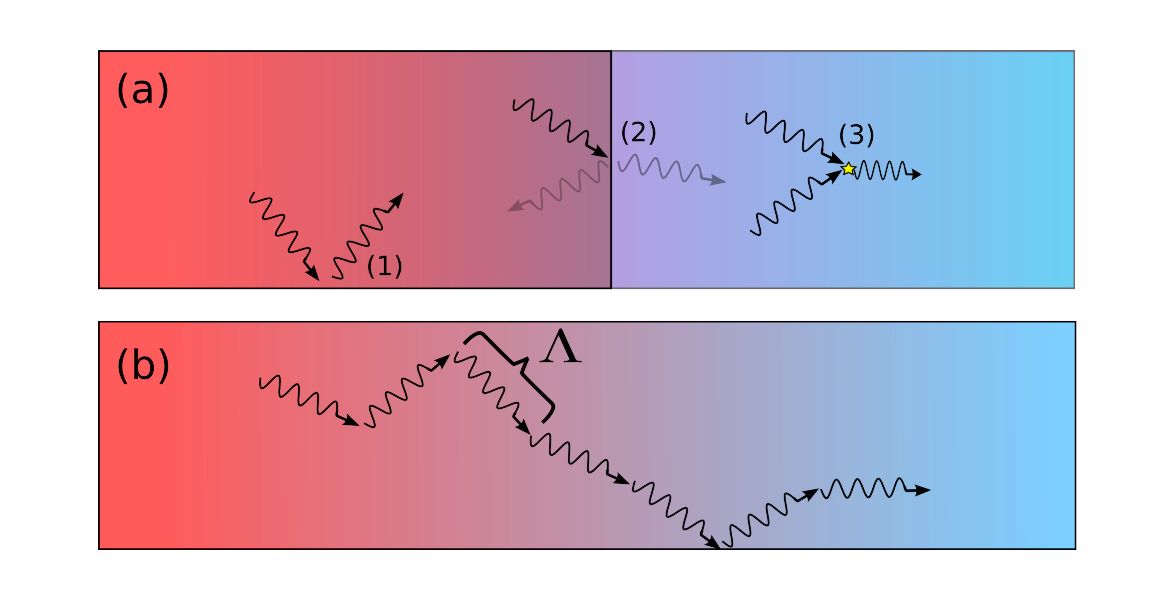
\includegraphics[width=.99\columnwidth]{inkscape/scattering.pdf}
 \caption{(a) Schematic illustration of microscopic phonon scattering mechanisms considered in this work: (1) Boundary scattering, (2) interface scattering, (3) phonon-phonon scattering. (b) Schematic of phonon propagation in a material, with scattering events at average distances of mean free path $\Lambda$.}
\label{fig:intro_scattering}
\end{center}
\end{figure}

The characteristic distance between phonon scattering events is called the phonon mean free path. While phonon mean free paths depend strongly on the material, temperature, vibrational frequency, and the type of scattering (elastic versus inelastic), a typical value for bulk silicon is around $\sim 300$ nm at room temperature \cite{ju99}. At length scales smaller than the mean free path, scattering events are too infrequent to drive phonon gas to local thermal equilibrium. Consequently, the classical Fourier's law of conduction \cite{fourier} based on the concept of a well-defined local temperature and equilibrium breaks down. 

Because of the relatively long intrinsic phonon mean free paths and the high surface-to-volume ratio of nanostructures, material interfaces and surfaces often have a dominant contribution to thermal resistance. Microscopically, phonon scattering at the interface between dissimilar materials arises both from atomic disorder at the interface and from the mismatch in the acoustic properties of the materials \cite{khalatnikov52}. Interfacial thermal resistance can present a bottleneck for the extraction of generated heat in electronic devices, thereby limiting their performance \cite{pop10,moore14}. Many methods have been suggested to reduce the thermal resistance between materials, including chemical functionalization \cite{hopkins11,kaur14,han15b}, external pressure \cite{shen11,chalopin12}, heat-mediating thin films \cite{english12}, and surface patterning \cite{merabia14}. 

In a similar way, boundary scattering from material surfaces can strongly reduce the thermal conductivity in nanowires and thin films. Because efficient conversion of waste heat to electricity requires materials with a low thermal conductivity (and high electrical conductivity) \cite{chen}, low-dimensional materials such as silicon nanowires have been suggested to provide attractive platforms for thermoelectric modules \cite{hochbaum08,boukai08}. To reduce the thermal conductivity of nanowires even further, additional structuring such as alloying \cite{garg11}, partial amorphization \cite{donadio09}, coating \cite{hu11}, and superlattice structures \cite{hu12} have been suggested.

Efficient extraction of heat from electronic devices requires not only small interfacial resistances but also materials that can efficiently carry heat away from the device \cite{pop10}. Carbon nanotubes  \cite{iijima91} are good candidates for such thermal management \cite{kumar11} because of their high thermal conductivity in the range of 500-5000 W/(mK) \cite{marconnet13}. Because of the very long phonon mean free paths of carbon nanotubes, the thermal conductivity depends on the tube length in tubes as long as 5 $\upmu$m \cite{chang08}. It is, however, unclear whether ballistic conduction extends to millimeter-long tubes \cite{marconnet13}. It is even possible that the thermal conductivity of pristine carbon nanotubes diverges as a function of tube length, revealing a signature of anomalous thermal conduction observed in computer simulations for one-dimensional atomic chains \cite{lepri03,mai07,dhar08}. Indications of anomalous thermal conduction were recently observed experimentally \cite{xu14} for graphene, the two-dimensional allotrope of carbon.

For applications in thermionic \cite{zeng06,westover08} and thermophotonic \cite{oksanen10} cooling as well as thermophotovoltaic generation \cite{dimatteo01}, good thermal insulation between materials separated by nanoscale gap is required. Nanoscale point contacts bridging the vacuum gap and providing structural support are a good alternative due to their small thermal conductance \cite{bartsch12}. In such small structures, interference effects arising from the wave nature of phonons cannot be neglected. While earlier works have investigated the thermal conductance of point contacts \cite{bartsch12,jeong12}, they have not specifically addressed the interference effects. Recognizing interference effects in point contacts could enable thermal conductivity engineering in a similar way as, e.g., in silicon thin films decorated with local resonators \cite{davis14}.

\subsection{Electromagnetic energy transfer in the near-field}
\label{sec:intro_em}

Unlike lattice vibrations, electromagnetic fields can propagate and transfer heat even in vacuum. This phenomenon is best observed on a sunny day when the electromagnetic radiation emitted from the Sun heats the skin. Like Sun, any object at non-zero temperature emits thermal radiation with a wide spectrum of wavelengths. According to Wien's law \cite{modest}, the spectrum of emitted thermal radiation peaks at a wavelength $\lambda_{\textrm{max}}$ that is inversely proportional to the object's temperature $T$. While $\lambda_{\textrm{max}}$ is around 500 nm for the Sun (with surface temperature $T\approx 5800$ K), objects at room temperature have the peak wavelength at $\lambda_{\textrm{max}}\approx 10$ $\upmu$m, corresponding to infrared radiation. 

\begin{figure}
\begin{center}
 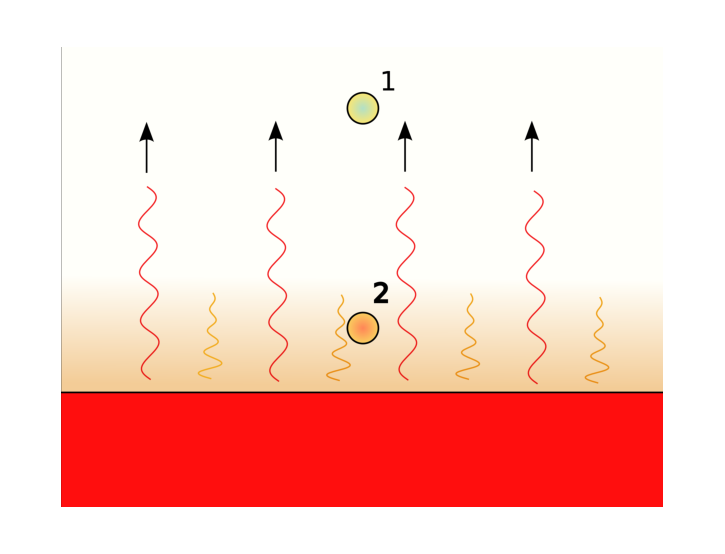
\includegraphics[width=.80\columnwidth]{inkscape/thermal_radiation.pdf}
 \caption{Due to microscopic thermal fluctuations, a body at non-zero temperature (red block) emits thermal radiation in the form of propagating electromagnetic waves (red wavy lines), which can carry energy to another object in the far-field (1). Close to the radiating body, there are, however, also evanescent waves (orange wavy lines) with zero propagation velocity. For an object placed in the near-field (2), the evanescent waves can enhance the energy transfer from the radiating body by orders of magnitude compared to the far-field value.}
\label{fig:intro_em}
\end{center}
\end{figure}

Thermal electromagnetic field generated by any object generally consists of propagating waves (''far-field'') and evanescent waves (''near-field'') \cite{novotny}. At small distances from the emitting body, evanescent waves typically dominate the electromagnetic energy density and can thereby strongly increase the energy transfer rates compared to the far-field value, as depicted in Fig. \ref{fig:intro_em}. Because evanescent waves are localized roughly at distances smaller than $\lambda_{\textrm{max}}$ from the surface of the object, their contribution to room-temperature energy transfer is typically notable at submicron distances.

The near-field enhancement of energy transfer was first observed by Hargreaves \cite{hargreaves69}, who measured the thermal conductance between two chromium layers separated by a micrometer-scale gap. The theoretical calculation for the exact enhancement rate was carried out by Polder and van Hove \cite{polder71}, and consequently near-field enhancement effects were predicted in numerous geometries \cite{loomis94,pendry99,carminati99,shchegrov00,mulet01,volokitin01}. In the last decade, advances in experimental techniques have allowed for very precise measurements of near-field enhancement rates \cite{kittel05,hu08,shen09,ottens11}, confirming theoretical predictions. 

In addition to existing applications in, e.g., thermal microscopy \cite{majumdar99,muller-hirsch99,kittel05,kittel08} and thermophotovoltaics \cite{dimatteo01,narayanaswamy03,laroche06}, near-field effects are expected to be exploitable also in nanoscale thermal management, with possible applications in heat-assisted chemistry \cite{cao07,adleman09} and hyperthermic treatment of cancer \cite{vanderzee02}. The strong near-field interaction allows, for example, for the quick dissipation of heat from a heated nanoparticle to its near surroundings \cite{mulet01,domingues05}. Because of the short-ranged nature of the near-field, the enhanced coupling is, however, limited to very small distances. It has been suggested that thermal coupling between bodies could be further enhanced by the introduction of additional nanoparticles  \cite{benabdallah11,messina13} or heat-mediating thin films \cite{zheng11,messina12}. 

\subsection{Computational modeling of electronic effects in energy transfer}
\label{sec:intro_electrons}

Exponential increase in the density of transistors in state-of-the-art microchips has strongly increased the power dissipated by CPUs, increasing their power consumption and requiring drastic cooling solutions in datacenters \cite{pop10}. Proper management of the unwanted heat at both chip and individual transistor level is therefore a key ingredient of modern electronics design \cite{moore14}. Nanostructures are considered attractive platforms for thermal management due to their possibly superior performance as heat-spreading layers and thermal interface materials \cite{moore14}. 

Numerical simulations are generally needed to model the electron-phonon coupling responsible for heat generation in nanoelectronic devices \cite{pop06_ieee}. Computational modeling of electron-phonon interactions in complex systems has been mainly carried out by Monte Carlo simulations and classical two-temperature models (see, e.g., Refs. \cite{chen01,chen06,sadi06,guo12} and references therein), which both neglect the wave nature of electrons and phonons and are therefore of limited use in, e.g., quantum well or dot structures with feature sizes below 10 nm. First-principles modeling of electron-phonon coupling \cite{luisier09} is, on the other hand, computationally heavy and therefore restricted to simple structures.

Langevin theory \cite{dhar03,roy07,jacquet09} is a promising alternative for the efficient modeling of dissipative electron transfer in atomistic scale. Despite its applicability to complex structures, Langevin theory has only been applied to simple toy systems so far. Langevin modeling of transport is described in detail in Chap. \ref{chap:theory}, where we highlight the close correspondence between the Langevin models of electron, phonon and photon transfer. 

\section{Studied structures}

\begin{figure}
\begin{center}
 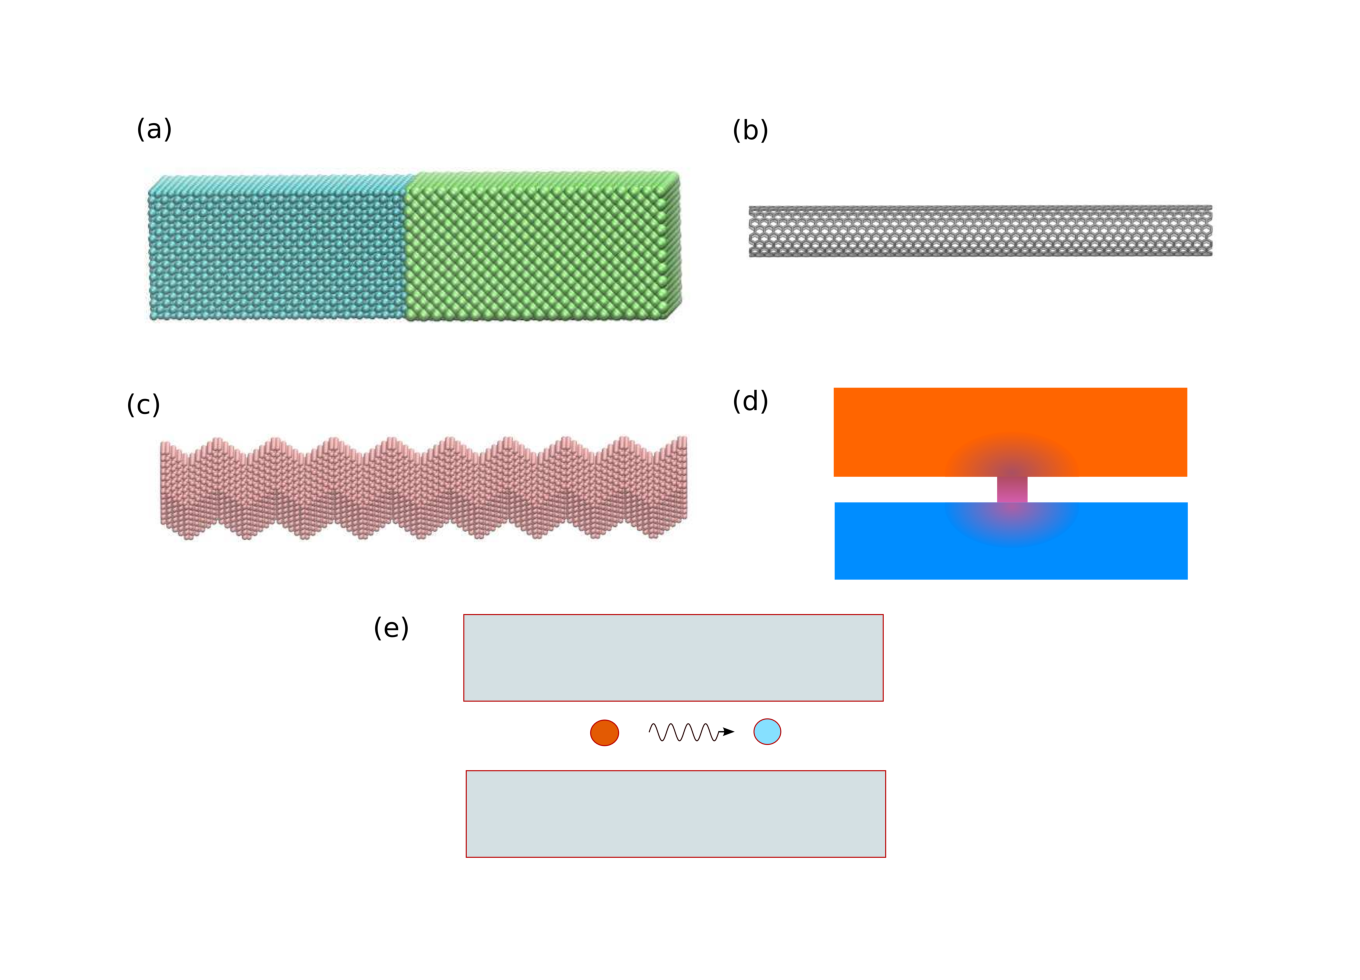
\includegraphics[width=1\columnwidth]{inkscape/systems.pdf} 
 \caption{Schematic illustration of the structures investigated in this work: (a) An interface between two crystals with different atomic masses, (b) a carbon nanotube, (c) a silicon nanowire with periodic twinning, (d) a point contact connecting bulk materials, and (e) two nanoparticles interacting electromagnetically in a mirror cavity. Atomistic illustrations of (a), (b), and (c) were prepared using the VMD visualization software \cite{humphrey96}.}
\label{fig:intro_structures}
\end{center}
\end{figure}

The structures investigated in the publications of this thesis are depicted in Fig. \ref{fig:intro_structures}. The broad topics concerning each depicted structure were, corresponding to figure labeling, (a) interfacial thermal resistance, (b) phonon mean free paths in nanotubes, (c) thermal conductivity engineering in nanowires, (d) phonon interference effects in point contacts, and (e) electromagnetic energy transfer in microcavities. 

The interface structure of Fig. \ref{fig:intro_structures}(a) is used as the simulation geometry to study the role of phonon-phonon scattering in interfacial thermal conduction between two bulk crystals with different masses. The results of \citepub{spectral} show that phonon-phonon scattering can reduce the resistance via two mechanisms, namely (1) dissipation of evanescent vibrational modes localized close to the interface, and (2) energy-doubling and energy-halving three-phonon scattering processes carrying energy across the interface.  

The carbon nanotube structure schematically depicted in Fig. \ref{fig:intro_structures}(b) is used in the simulations of \citepub{cnt} to determine the phonon mean free paths in carbon nanotubes. The mean free paths were determined from non-equilibrium simulations by utilizing the spectral analysis methods developed in \citepub{spectral}. The mean free paths in carbon nanotubes were shown to exceed 10 $\upmu$m at low frequencies, with possibly even longer mean free paths at lower frequencies. The results suggest that even very long nanotubes approaching the millimeter-scale can exhibit partially ballistic thermal conduction at room temperature. 

Figure \ref{fig:intro_structures}(c) shows a silicon nanowire with periodic twinning stacking faults, which create a zigzag-like structure impeding phonon flow and thereby reducing thermal conductivity compared to the straight wire. The atomistic simulations of \citepub{twinning} show that periodic twinning can reduce the thermal conductivity of Si nanowires by 65 \% at room temperature, suggesting that twinning could boost the thermoelectric efficiency of silicon nanowires. Twinning can also be paired with other structural modifications to reduce the thermal conductivity even further.

Thermal conduction through a nanoscale point contact, illustrated in Fig. \ref{fig:intro_structures}(d), is the topic of Publications \cp{fpu}, \cp{fpu2}, and \cp{gf}. For a point contact in a square lattice, interference effects are shown to give rise to directional features in the local temperature profile. As expected, interference features are washed away at higher temperature because of the increasing phonon-phonon scattering. Local temperature profile is also modified when the quantum-mechanical occupation function of heat carriers is taken into account. 

Figure \ref{fig:intro_structures}(e) illustrates two polar nanoparticles located in a microcavity. The calculations of \citepub{dipole} show that the cavity (i) increases the thermal coupling between nanoparticles and (ii) gives rise to non-monotonic thermal coupling as a function of nanoparticle distance arising from the interference of the standing cavity waves. The results suggest that modifying the electromagnetic environment can be used to flexibly and efficiently tune the thermal coupling between electromagnetically coupled bodies.


